% !TEX encoding = UTF-8
% !TEX TS-program = pdflatex
% !TEX root = ../tesi.tex


\chapter{Tools and applications}
	\section{Network Simulator 3}
		\label{sec:ns3}
		Network Simulator 3 (ns-3) is a discrete-event network simulator for Internet systems, targeted primarily for research and educational use. ns-3 is free software, licensed under the GNU GPLv2 license, and is publicly available for research, development, and use.
		
		
		ns-3 development began in 2006 by a team lead by Tom Henderson, George Riley, Sally Floyd and Sumit Roy. Its first version was released on June 30, 2008. 
		
		
		ns-3 is the successor of ns-2, released in 1989. The fact that the former was built from scratch makes it impossible to have backward compatibility. In fact, ns-2 used oTCL scripting language to describe network topologies and C++ to write the core of the simulation. This choice was due to avoid the very time consuming C++ code recompilation, exploiting the interpreted language oTCL. ns-2 mixed the \jquote{fast to run, slow to change} C++ with the \jquote{slow to run, fast to change} oTCL language. Since compilation time was not an issue with modern computing capabilities, ns-3 developers chose to utilize exclusively C++ code (and optional Python bindings) to develop simulations.
		
		\subsection{Modules and module structure}
		ns-3 is composed of various modules, which are groups of classes, examples and tests each related to a certain feature. The components of a module work in a cohesive way in order to offer APIs to other modules and users. Some examples of built-in modules are:
		\begin{itemize}
			\item WiFi;
			\item AODV; 
			\item CSMA.
		\end{itemize}
		The obstacle shadowing propagation loss model and the Fast-Broadcast and ROFF algorithms have been implemented as modules too.
		
		
		Modules follow a prototypical structure in order to promote clarity and offer built-in documentation. \imgrefcap{fig:ns-3-module} shows the typical module structure.
		
		\begin{figure}[H]
			\centering
			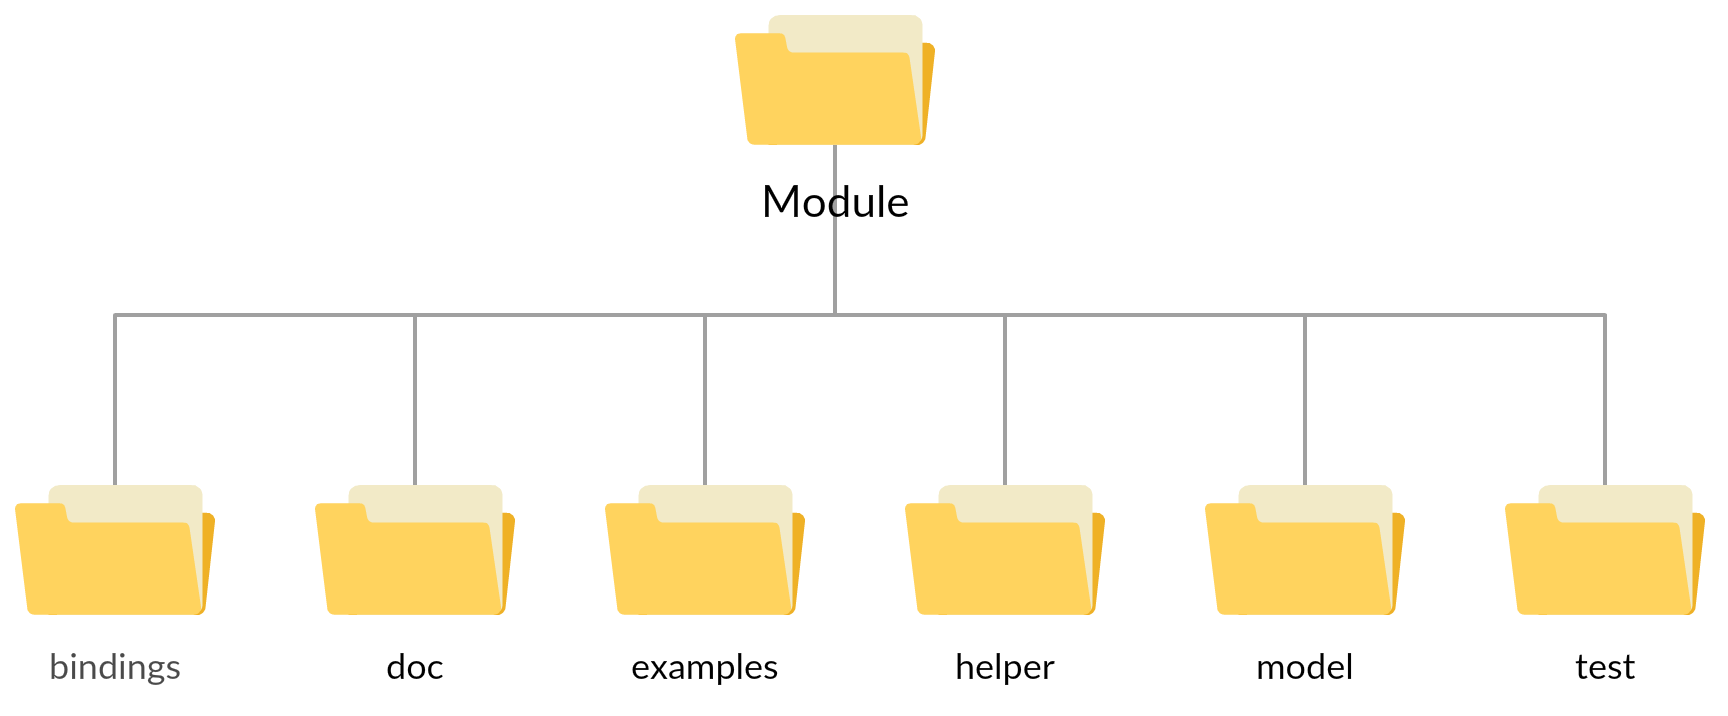
\includegraphics[width=\textwidth]{immagini/ns-3-module}
			\caption{ns-3 module structure}
			\label{fig:ns-3-module}
		\end{figure}
		
		The following directories can be found inside a module's root directory:
		\begin{itemize}
			\item \textbf{bindings:} Python bindings used to make the module's API compatible with Python;
			\item \textbf{doc:} documentation of the module;
			\item \textbf{examples:} examples and proof of concepts of what can be done using the module;
			\item \textbf{helper:} higher level APIs to make the module easier to use;
			\item \textbf{model:} headers and source files which implement the module's logic; 
			\item \textbf{test:} test suite and test cases to test the module.
		\end{itemize}
	
		\subsection{Key elements}
			The element at the base of ns-3 is called \textit{node}, instance of \texttt{ns3::Node}. A node can be thought of as a shell of a computer. Various other elements can be added to nodes, such as:
			\begin{itemize}
				\item NetDevices (e.g. \acrshort{nica}s, which enable nodes to communicate over \textit{channels});
				\item protocols;
				\item applications. 
			\end{itemize}
			The applications implement the logic of a simulation. For example, the \texttt{UdoEchoClientApplication} and \texttt{UdpEchoServerApplication} can be used to implement a client/server application which exchange and print the packets' content over the network.
			
		
		The \textit{channels} model various type of transmission media, such as the wired and the wireless ones.
	
		\subsection{Structure of a simulation}
			A simulation can be implemented in many ways, but in most cases the following steps are executed:
			\begin{itemize}
				\item manage command line arguments (e.g. number of nodes to consider in the simulation, transmission range, etc.);
				\item initialize all the necessary fields in classes;
				\item create nodes;
				\item set up physical and MAC layers;
				\item set up link layer, routing protocols and addresses;
				\item configure and install applications on nodes;
				\item position nodes and (optionally) give them a mobility model;
				\item schedule user defined events, such as transmissions of packets;
				\item start the simulation;
				\item collect and manage output data.
			\end{itemize}
		
		\subsection{NetAnim}
			Netanim is an offline animator tool based on the Qt toolkit. It collects an XML tracefile during the execution of a simulation and can be used to animate the simulation, analyzing packet transmissions and contents.
			
			\begin{figure}[H]
				\centering
				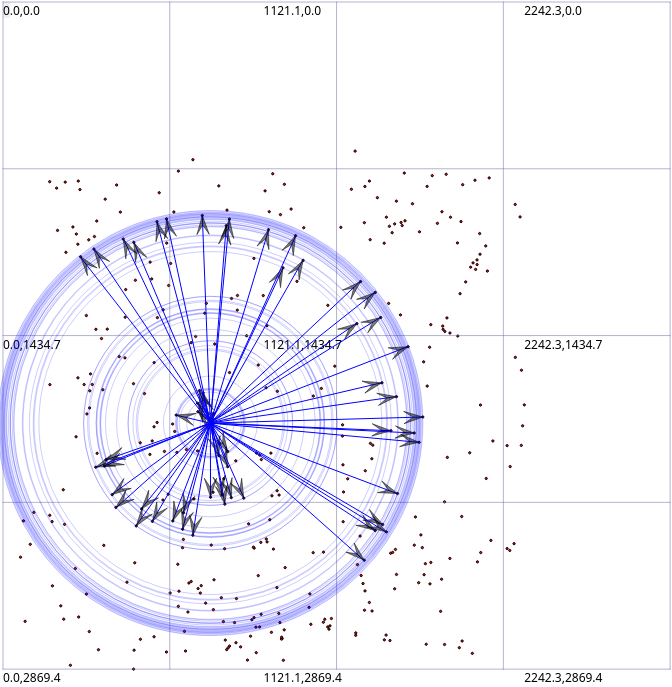
\includegraphics[scale=0.38]{immagini/netanim}
				\caption{Packet transmission in NetAnim}
				\label{fig:netanim}
			\end{figure}
	
	\section{Simulation of Urban MObility}
		\label{sec:sumo}
		Simulation of Urban MObility is an open-source road traffic simulation package. It is written in C++ and licensed under GPLv3. 
		
		
		It offers different tools to analyze and manage real maps from the urban mobility point of view, including pedestrian movement and various types of vehicles.
		
		
		The original work \cite{ROM2017} , starting from real maps obtained from OpenStreetMap (OSM), utilized SUMO to produce two files:
		\begin{enumerate}
			\item a \texttt{.poly} file using the SUMO tool \textit{Polyconvert}. This file contains information about all the obstacles, such as buildings, useful for the Obstacle Shadowing module;
			\item a \texttt{.ns2mobility} file using the SUMO tool \textit{TraceExporter}. This file contains information about the vehicles and their positioning. 
		\end{enumerate}
		The process of generating these two files necessary for ns-3 simulations requires some intermediate steps. The full process is represented in Figure \ref{fig:sumo-process}. 
		
		The original work considered a only a distance of 25 meters between vehicles; this work considers various distances, ranging from 5 to 45 meters. Figure \ref{fig:sumo-distances}  shows the same scenario (Padua) with different distances between vehicles.
		
		
		One of the intermediate results, the \texttt{.net} file which describes the road infrastructure using a graph resulting from \textit{Netconvert}, has been utilized for junction modeling, as explained in Section \ref{sec:junction-modeling}.
		\begin{figure}[H]
			\centering
			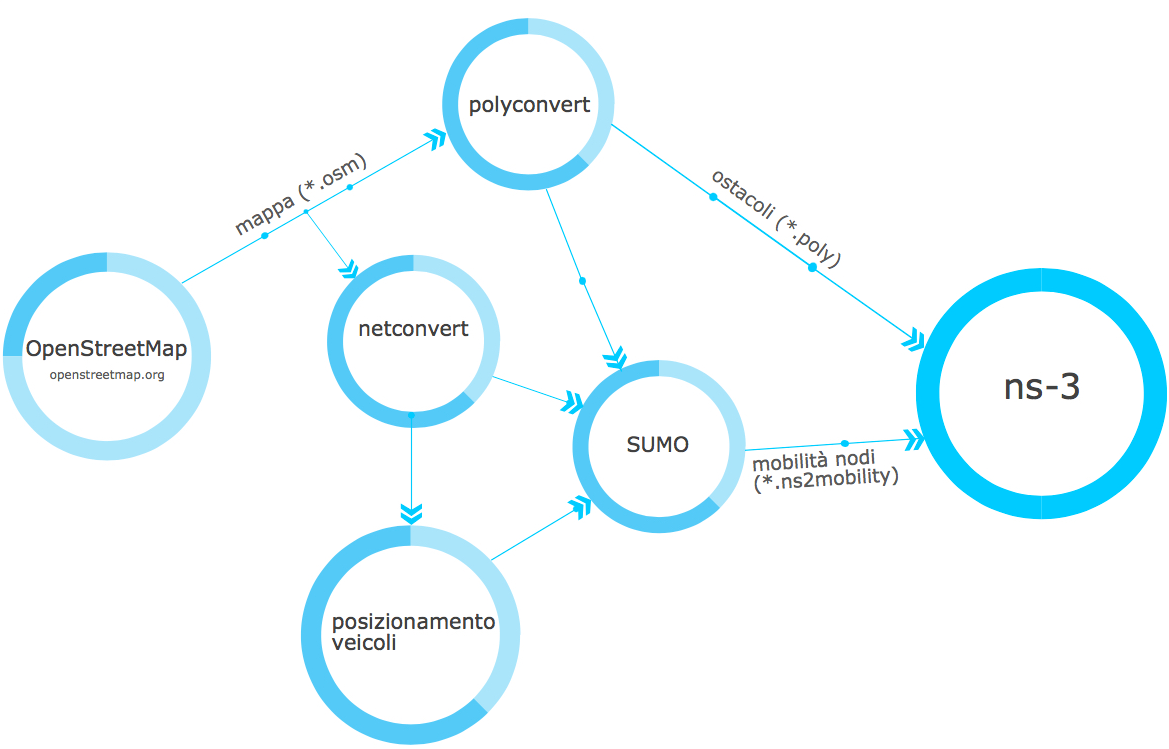
\includegraphics[width=\textwidth]{immagini/sumo-process}
			\caption{Steps to generate necessary files using SUMO (\cite{ROM2017})}
			\label{fig:sumo-process}
		\end{figure}
		
		\begin{figure}[H]
			\centering
			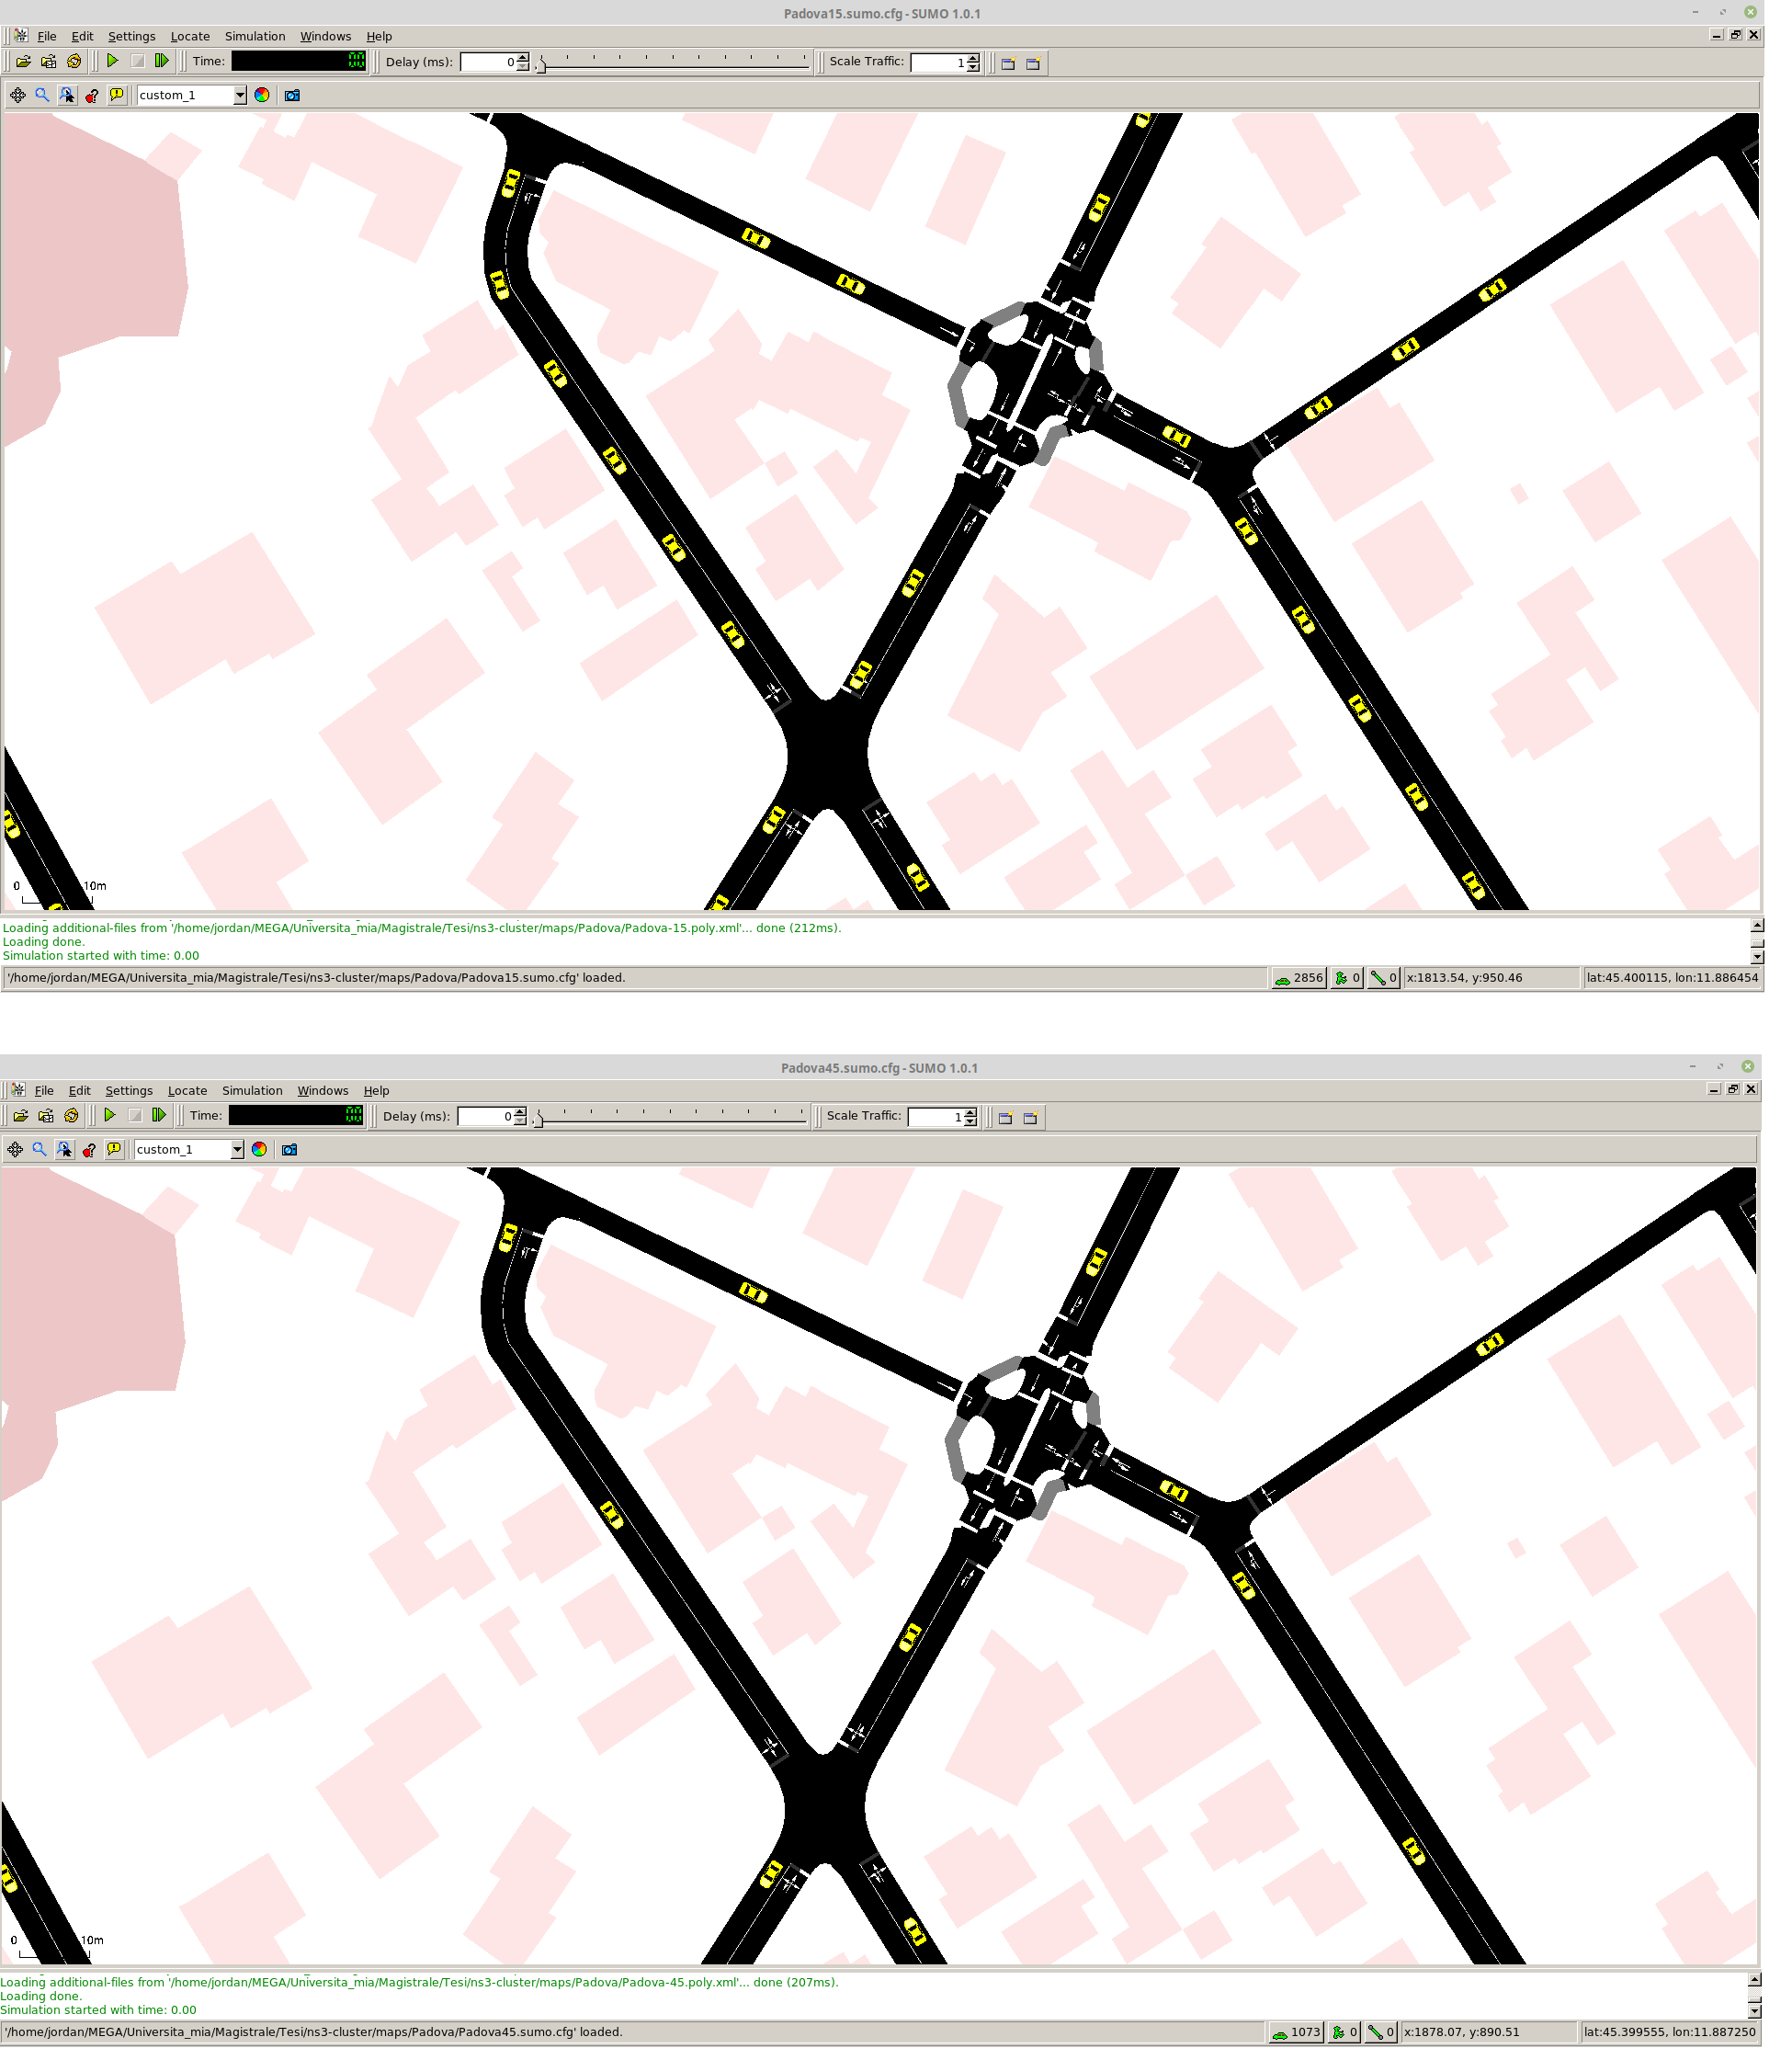
\includegraphics[width=\textwidth]{immagini/sumo-distances}
			\caption{Padua scenario with vehicle distance equals to 15 meters (top) and 45 meters (bottom)}
			\label{fig:sumo-distances}
		\end{figure}
